%%% APPENDIX
\chapter{Appendix}\label{chap:appendix}


\section[Vavilov vs Landau distribution]{On the Vavilov distribution approximation}\label{sec:vavilov_vs_landau_distribution}

% \cite[189]{NAP20066}
%     
% \maketitle
    
\begin{tcolorbox}[breakable, size=fbox, boxrule=1pt, pad at break*=1mm,colback=cellbackground, colframe=cellborder]
\prompt{In}{incolor}{1}{\boxspacing}
\begin{Verbatim}[commandchars=\\\{\}]
\PY{k+kn}{import} \PY{n+nn}{numpy} \PY{k}{as} \PY{n+nn}{np} \PY{c+c1}{\PYZsh{} NumPy}
\PY{k+kn}{from} \PY{n+nn}{scipy}\PY{n+nn}{.}\PY{n+nn}{optimize} \PY{k+kn}{import} \PY{n}{fsolve} 
\PY{k+kn}{from} \PY{n+nn}{IPython}\PY{n+nn}{.}\PY{n+nn}{display} \PY{k+kn}{import} \PY{n}{Image}
\PY{k+kn}{import} \PY{n+nn}{pandas} \PY{k}{as} \PY{n+nn}{pd} \PY{c+c1}{\PYZsh{} Pandas}
\PY{n}{pd}\PY{o}{.}\PY{n}{options}\PY{o}{.}\PY{n}{display}\PY{o}{.}\PY{n}{float\PYZus{}format} \PY{o}{=} \PY{l+s+s1}{\PYZsq{}}\PY{l+s+si}{\PYZob{}:5,.4E\PYZcb{}}\PY{l+s+s1}{\PYZsq{}}\PY{o}{.}\PY{n}{format}
\end{Verbatim}
\end{tcolorbox}

    \hypertarget{calculating-the-factor-the-determines-if-the-vavilov-distribution-can-be-approximated-by-a-landau}{%
\section{Calculating the factor the determines if the Vavilov
distribution can be approximated by a
Landau}\label{calculating-the-factor-the-determines-if-the-vavilov-distribution-can-be-approximated-by-a-landau}}

Bethe-Bloch mean energy loss: \[
\left\langle-\frac{dE}{dx} \right\rangle \frac{1}{\rho} =  K z_0^2 \frac{1}{\beta^2} \frac{Z}{A M_u} \cdot\left[\frac{1}{2}\ln \left(\frac{2m_e c^2 \beta^2 W_{max}}{I^2 \cdot (1-\beta^2)}\right) - \beta^2\right]
\]

\[
K/M_u = 4 \pi N_A r_e^2 m_e c^2 /M_u = 0.307075\space \text{MeV g}^{-1} \text{cm}^2
\]

\[
r_e  = \frac{e^2}{4\pi\varepsilon_0 m_e c^2} \\
M_u = 1 \frac{g}{mol} \quad z_0=1 \\
\left( W_{max} \equiv \epsilon_{max} \right)
\]

For \textbf{silicon}: \[
Z = 14 \\
A = 28.085 \\ 
\rho = 2.329085 \text{  g cm}^{-3}\\
I = 173 \text{ eV} % \quad \text{(mean excitation energy)}
\]

\hypertarget{calculating-beta-for-a-proton-of-energy-e_k}{%
\subsubsection{\texorpdfstring{Calculating \(\beta\) for a proton of
energy
\(E_k\)}{Calculating \textbackslash beta for a proton of energy E\_k}}\label{calculating-beta-for-a-proton-of-energy-e_k}}

\[
E_k = (\gamma - 1) m_o c^2 \\
\gamma = \frac{E_k + m_o c^2}{m_o c^2} \\
\beta^2 = 1 - \left(\frac{m_o c^2}{E_k +m_o c^2} \right)^2
\]

for a proton of energy \(E_k=120\space \text{GeV}\),
\(m_0 = 938.272\space \text{MeV/c}^2\)

    \begin{tcolorbox}[breakable, size=fbox, boxrule=1pt, pad at break*=1mm,colback=cellbackground, colframe=cellborder]
\prompt{In}{incolor}{2}{\boxspacing}
\begin{Verbatim}[commandchars=\\\{\}]
\PY{n}{energy} \PY{o}{=} \PY{l+m+mf}{120e3} \PY{c+c1}{\PYZsh{} MeV  (120 GeV)}
\PY{c+c1}{\PYZsh{} m\PYZus{}particle = 938.272088 \PYZsh{} MeV/c\PYZca{}2  protons }
\PY{n}{m\PYZus{}particle} \PY{o}{=} \PY{l+m+mf}{938.213} \PY{c+c1}{\PYZsh{} MeV/c\PYZca{}2     protons (older value)}

\PY{n}{gamma} \PY{o}{=} \PY{p}{(}\PY{n}{energy} \PY{o}{+} \PY{n}{m\PYZus{}particle}\PY{p}{)}\PY{o}{/}\PY{n}{m\PYZus{}particle}
\PY{n}{beta\PYZus{}2} \PY{o}{=} \PY{l+m+mi}{1} \PY{o}{\PYZhy{}} \PY{n}{m\PYZus{}particle}\PY{o}{*}\PY{o}{*}\PY{l+m+mi}{2}\PY{o}{/}\PY{p}{(}\PY{n}{m\PYZus{}particle} \PY{o}{+} \PY{n}{energy}\PY{p}{)}\PY{o}{*}\PY{o}{*}\PY{l+m+mi}{2}

\PY{n+nb}{print}\PY{p}{(}\PY{l+s+s2}{\PYZdq{}}\PY{l+s+s2}{ gamma: }\PY{l+s+s2}{\PYZdq{}}\PY{p}{,} \PY{n}{gamma}\PY{p}{,} \PY{l+s+s2}{\PYZdq{}}\PY{l+s+se}{\PYZbs{}n}\PY{l+s+s2}{\PYZdq{}}\PY{p}{,} \PY{l+s+s2}{\PYZdq{}}\PY{l+s+s2}{beta²: }\PY{l+s+s2}{\PYZdq{}}\PY{p}{,} \PY{n}{beta\PYZus{}2}\PY{p}{)}
\end{Verbatim}
\end{tcolorbox}

    \begin{Verbatim}[commandchars=\\\{\}]
 gamma:  128.90272571367058
 beta²:  0.999939816727599
    \end{Verbatim}

    from https://academic.oup.com/book/43645/chapter/365027598\#404941541 :

The parameter \(\kappa\) of the Vavilov distribution determines if it
becomes close to a Landau (\(\kappa\rightarrow0\)) or a Gaussian
(\(\kappa 10\)).

To calculate \(\kappa\): 
\[
\kappa = \frac{\xi}{\epsilon_{max}}
\]

where: \[
\xi = \frac{1}{2} K \frac{Z}{A} \frac{s} {\beta^2}
\]

\(s = \Delta x \cdot \rho\)

and from https://nap.nationalacademies.org/read/20066/chapter/10\#188 :
\[
\epsilon_{max} = \frac{2m_e c^2 \beta^2}{1-\beta^2}\left[ 1 + \frac{2m_e}{M}\frac{1}{\sqrt{1-\beta^2}} + \left(\frac{m_e}{M}\right)^2 \right]^{-1}
\]

where \(M\) is the mass of the incoming particle.

Also written as:

\[
\epsilon_{max} = \frac{2m_e c^2 \beta^2 \gamma^2} { 1 + \frac{2\gamma m_e}{M} + \left(\frac{m_e}{M}\right)^2}
\]

    \hypertarget{applying-this-to-a-thin-silicon-layer-50mu-textm}{%
\subsubsection{\texorpdfstring{Applying this to a thin silicon layer
(50\(\mu \text{m}\))}{Applying this to a thin silicon layer (50\textbackslash mu \textbackslash text\{m\})}}\label{applying-this-to-a-thin-silicon-layer-50mu-textm}}

(The masses are either multiplied by \(c^2\) or in a ratio, the mass
units used are \(\text{MeV}/c^2\))

    \begin{tcolorbox}[breakable, size=fbox, boxrule=1pt, pad at break*=1mm,colback=cellbackground, colframe=cellborder]
\prompt{In}{incolor}{3}{\boxspacing}
\begin{Verbatim}[commandchars=\\\{\}]
\PY{c+c1}{\PYZsh{}\PYZsh{}\PYZsh{} variables values}
\PY{n}{m\PYZus{}electron} \PY{o}{=} \PY{l+m+mf}{0.51099895} \PY{c+c1}{\PYZsh{} MeV/c\PYZca{}2}
\PY{n}{z\PYZus{}0} \PY{o}{=} \PY{l+m+mi}{1} \PY{c+c1}{\PYZsh{} electric charge of incoming particle}
\PY{n}{delta\PYZus{}x} \PY{o}{=} \PY{l+m+mf}{5e\PYZhy{}3} \PY{c+c1}{\PYZsh{} cm  (50um)}

\PY{c+c1}{\PYZsh{}\PYZsh{}\PYZsh{} silicon}
\PY{n}{Z} \PY{o}{=} \PY{l+m+mi}{14}   \PY{c+c1}{\PYZsh{} atomic number}
\PY{n}{A} \PY{o}{=} \PY{l+m+mf}{28.085}  \PY{c+c1}{\PYZsh{} atomic weight}
\PY{n}{density} \PY{o}{=} \PY{l+m+mf}{2.329085} \PY{c+c1}{\PYZsh{} g cm\PYZca{}\PYZhy{}3}
\PY{n}{mean\PYZus{}excitation} \PY{o}{=} \PY{l+m+mf}{173e\PYZhy{}6} \PY{c+c1}{\PYZsh{} MeV  (mean excitation energy of Silicon: 173 eV)}

\PY{n}{s} \PY{o}{=} \PY{n}{delta\PYZus{}x} \PY{o}{*} \PY{n}{density} \PY{c+c1}{\PYZsh{} g cm\PYZca{}\PYZhy{}2}
\PY{n}{K} \PY{o}{=} \PY{l+m+mf}{0.307075} \PY{c+c1}{\PYZsh{} MeV g\PYZca{}\PYZhy{}1 cm\PYZca{}2}
\end{Verbatim}
\end{tcolorbox}

    \begin{tcolorbox}[breakable, size=fbox, boxrule=1pt, pad at break*=1mm,colback=cellbackground, colframe=cellborder]
\prompt{In}{incolor}{4}{\boxspacing}
\begin{Verbatim}[commandchars=\\\{\}]
\PY{k}{def} \PY{n+nf}{xi\PYZus{}func}\PY{p}{(}\PY{n}{energy}\PY{p}{)}\PY{p}{:}
    \PY{n}{beta\PYZus{}2} \PY{o}{=} \PY{l+m+mi}{1} \PY{o}{\PYZhy{}} \PY{n}{m\PYZus{}particle}\PY{o}{*}\PY{o}{*}\PY{l+m+mi}{2}\PY{o}{/}\PY{p}{(}\PY{n}{m\PYZus{}particle} \PY{o}{+} \PY{n}{energy}\PY{p}{)}\PY{o}{*}\PY{o}{*}\PY{l+m+mi}{2}
    \PY{k}{return} \PY{p}{(}\PY{l+m+mi}{1}\PY{o}{/}\PY{l+m+mi}{2} \PY{o}{*} \PY{n}{K}\PY{p}{)} \PY{o}{*} \PY{p}{(}\PY{n}{Z} \PY{o}{/} \PY{n}{A}\PY{p}{)} \PY{o}{*} \PY{p}{(}\PY{n}{s} \PY{o}{/} \PY{n}{beta\PYZus{}2}\PY{p}{)}

\PY{k}{def} \PY{n+nf}{eps\PYZus{}max\PYZus{}func}\PY{p}{(}\PY{n}{energy}\PY{p}{)}\PY{p}{:}
    \PY{n}{gamma} \PY{o}{=} \PY{p}{(}\PY{n}{energy} \PY{o}{+} \PY{n}{m\PYZus{}particle}\PY{p}{)}\PY{o}{/}\PY{n}{m\PYZus{}particle}
    \PY{n}{beta\PYZus{}2} \PY{o}{=} \PY{l+m+mi}{1} \PY{o}{\PYZhy{}} \PY{n}{m\PYZus{}particle}\PY{o}{*}\PY{o}{*}\PY{l+m+mi}{2}\PY{o}{/}\PY{p}{(}\PY{n}{m\PYZus{}particle} \PY{o}{+} \PY{n}{energy}\PY{p}{)}\PY{o}{*}\PY{o}{*}\PY{l+m+mi}{2}
    \PY{k}{return} \PY{p}{(}\PY{l+m+mi}{2} \PY{o}{*} \PY{n}{m\PYZus{}electron} \PY{o}{*} \PY{n}{beta\PYZus{}2} \PY{o}{*} \PY{n}{gamma}\PY{o}{*}\PY{o}{*}\PY{l+m+mi}{2}\PY{p}{)} \PY{o}{/} \PY{p}{(}\PY{l+m+mi}{1} \PY{o}{+} \PY{l+m+mi}{2}\PY{o}{*}\PY{n}{gamma}\PY{o}{*}\PY{n}{m\PYZus{}electron}\PY{o}{/}\PY{n}{m\PYZus{}particle} \PY{o}{+} \PY{p}{(}\PY{n}{m\PYZus{}electron}\PY{o}{/}\PY{n}{m\PYZus{}particle}\PY{p}{)}\PY{o}{*}\PY{o}{*}\PY{l+m+mi}{2}\PY{p}{)} \PY{c+c1}{\PYZsh{} MeV}

\PY{k}{def} \PY{n+nf}{kappa\PYZus{}func}\PY{p}{(}\PY{n}{energy}\PY{p}{,} \PY{n}{kappa\PYZus{}value}\PY{o}{=}\PY{l+m+mf}{0.01}\PY{p}{)}\PY{p}{:}
    \PY{l+s+sd}{\PYZdq{}\PYZdq{}\PYZdq{}kappa as a function of the energy (to find the zeros for k=kappa\PYZus{}value)\PYZdq{}\PYZdq{}\PYZdq{}}
    \PY{n}{gamma} \PY{o}{=} \PY{p}{(}\PY{n}{energy} \PY{o}{+} \PY{n}{m\PYZus{}particle}\PY{p}{)}\PY{o}{/}\PY{n}{m\PYZus{}particle}
    \PY{n}{beta\PYZus{}2} \PY{o}{=} \PY{l+m+mi}{1} \PY{o}{\PYZhy{}} \PY{n}{m\PYZus{}particle}\PY{o}{*}\PY{o}{*}\PY{l+m+mi}{2}\PY{o}{/}\PY{p}{(}\PY{n}{m\PYZus{}particle} \PY{o}{+} \PY{n}{energy}\PY{p}{)}\PY{o}{*}\PY{o}{*}\PY{l+m+mi}{2}
    \PY{k}{return} \PY{n}{xi\PYZus{}func}\PY{p}{(}\PY{n}{energy}\PY{p}{)} \PY{o}{/} \PY{n}{eps\PYZus{}max\PYZus{}func}\PY{p}{(}\PY{n}{energy}\PY{p}{)} \PY{o}{\PYZhy{}} \PY{n}{kappa\PYZus{}value}
\end{Verbatim}
\end{tcolorbox}

    \begin{tcolorbox}[breakable, size=fbox, boxrule=1pt, pad at break*=1mm,colback=cellbackground, colframe=cellborder]
\prompt{In}{incolor}{5}{\boxspacing}
\begin{Verbatim}[commandchars=\\\{\}]
\PY{n}{xi} \PY{o}{=} \PY{p}{(}\PY{l+m+mi}{1}\PY{o}{/}\PY{l+m+mi}{2} \PY{o}{*} \PY{n}{K}\PY{p}{)} \PY{o}{*} \PY{p}{(}\PY{n}{Z} \PY{o}{/} \PY{n}{A}\PY{p}{)} \PY{o}{*} \PY{p}{(}\PY{n}{s} \PY{o}{/} \PY{n}{beta\PYZus{}2}\PY{p}{)} \PY{c+c1}{\PYZsh{} MeV}

\PY{n}{epsilon\PYZus{}max} \PY{o}{=} \PY{n}{eps\PYZus{}max\PYZus{}func}\PY{p}{(}\PY{n}{energy}\PY{p}{)} \PY{c+c1}{\PYZsh{} MeV}

\PY{n}{kappa} \PY{o}{=} \PY{n}{xi} \PY{o}{/} \PY{n}{epsilon\PYZus{}max}

\PY{n+nb}{print}\PY{p}{(}\PY{l+s+s2}{\PYZdq{}}\PY{l+s+s2}{k =}\PY{l+s+s2}{\PYZdq{}}\PY{p}{,}\PY{n}{kappa}\PY{p}{)}
\end{Verbatim}
\end{tcolorbox}

    \begin{Verbatim}[commandchars=\\\{\}]
k = 5.98637846070628e-08
    \end{Verbatim}

    \hypertarget{comparison-with-calculations-from-httpsnap.nationalacademies.orgread20066chapter10189}{%
\subsection{Comparison with calculations from \cite{NAP20066} }\label{comparison-with-calculations-from-httpsnap.nationalacademies.orgread20066chapter10189}}

    \begin{tcolorbox}[breakable, size=fbox, boxrule=1pt, pad at break*=1mm,colback=cellbackground, colframe=cellborder]
\prompt{In}{incolor}{6}{\boxspacing}
\begin{Verbatim}[commandchars=\\\{\}]
\PY{n}{Image}\PY{p}{(}\PY{l+s+s2}{\PYZdq{}}\PY{l+s+s2}{epsilon and xi formulas.png}\PY{l+s+s2}{\PYZdq{}}\PY{p}{,} \PY{n}{width}\PY{o}{=}\PY{l+m+mi}{1000}\PY{p}{)}
\end{Verbatim}
\end{tcolorbox}
 
            
\prompt{Out}{outcolor}{6}{}
    
    \begin{center}
    \adjustimage{max size={0.9\linewidth}{0.9\paperheight}}{Chapters/Vavilov_Landau/output_10_0.png}
    \end{center}
    { \hspace*{\fill} \\}
    

    Then follows a table with the values calculated for different energies:

    \begin{tcolorbox}[breakable, size=fbox, boxrule=1pt, pad at break*=1mm,colback=cellbackground, colframe=cellborder]
\prompt{In}{incolor}{7}{\boxspacing}
\begin{Verbatim}[commandchars=\\\{\}]
\PY{n}{Image}\PY{p}{(}\PY{l+s+s2}{\PYZdq{}}\PY{l+s+s2}{Table of k and xi values.png}\PY{l+s+s2}{\PYZdq{}}\PY{p}{,} \PY{n}{width}\PY{o}{=}\PY{l+m+mi}{800}\PY{p}{)}
\end{Verbatim}
\end{tcolorbox}
 
            
\prompt{Out}{outcolor}{7}{}
    
    \begin{center}
    \adjustimage{max size={0.9\linewidth}{0.9\paperheight}}{Chapters/Vavilov_Landau/output_12_0.png}
    \end{center}
    { \hspace*{\fill} \\}
    

    Comparison of these values with my previous calculations

    \begin{tcolorbox}[breakable, size=fbox, boxrule=1pt, pad at break*=1mm,colback=cellbackground, colframe=cellborder]
\prompt{In}{incolor}{8}{\boxspacing}
\begin{Verbatim}[commandchars=\\\{\}]
\PY{c+c1}{\PYZsh{} Values from 100 MeV to 10 GeV}
\PY{n}{energy\PYZus{}array} \PY{o}{=} \PY{n}{np}\PY{o}{.}\PY{n}{array}\PY{p}{(}\PY{p}{[}\PY{l+m+mi}{100}\PY{p}{,}\PY{l+m+mi}{150}\PY{p}{,}\PY{l+m+mi}{200}\PY{p}{,}\PY{l+m+mi}{300}\PY{p}{,}\PY{l+m+mi}{400}\PY{p}{,}\PY{l+m+mi}{500}\PY{p}{,}\PY{l+m+mi}{600}\PY{p}{,}\PY{l+m+mi}{800}\PY{p}{,}\PY{l+m+mi}{1000}\PY{p}{,}\PY{l+m+mi}{1500}\PY{p}{,}\PY{l+m+mi}{2000}\PY{p}{,}\PY{l+m+mi}{3000}\PY{p}{,}\PY{l+m+mi}{4000}\PY{p}{,}\PY{l+m+mi}{5000}\PY{p}{,}\PY{l+m+mi}{6000}\PY{p}{,}\PY{l+m+mi}{8000}\PY{p}{,}\PY{l+m+mi}{10000}\PY{p}{]}\PY{p}{)}
\end{Verbatim}
\end{tcolorbox}

    \begin{tcolorbox}[breakable, size=fbox, boxrule=1pt, pad at break*=1mm,colback=cellbackground, colframe=cellborder]
\prompt{In}{incolor}{9}{\boxspacing}
\begin{Verbatim}[commandchars=\\\{\}]
\PY{n}{table\PYZus{}data} \PY{o}{=} \PY{n}{np}\PY{o}{.}\PY{n}{vstack}\PY{p}{(}\PY{p}{(}\PY{l+m+mi}{1} \PY{o}{\PYZhy{}} \PY{n}{m\PYZus{}particle}\PY{o}{*}\PY{o}{*}\PY{l+m+mi}{2} \PY{o}{/} \PY{p}{(}\PY{n}{m\PYZus{}particle}\PY{o}{+}\PY{n}{energy\PYZus{}array}\PY{p}{)}\PY{o}{*}\PY{o}{*}\PY{l+m+mi}{2}\PY{p}{,}
              \PY{n}{eps\PYZus{}max\PYZus{}func}\PY{p}{(}\PY{n}{energy\PYZus{}array}\PY{p}{)}\PY{p}{,}
              \PY{n}{A}\PY{o}{/}\PY{n}{Z} \PY{o}{*} \PY{n}{xi\PYZus{}func}\PY{p}{(}\PY{n}{energy\PYZus{}array}\PY{p}{)} \PY{o}{/} \PY{n}{s}\PY{p}{,}
              \PY{n}{A}\PY{o}{/}\PY{n}{Z} \PY{o}{*} \PY{n}{kappa\PYZus{}func}\PY{p}{(}\PY{n}{energy\PYZus{}array}\PY{p}{,}\PY{n}{kappa\PYZus{}value}\PY{o}{=}\PY{l+m+mi}{0}\PY{p}{)} \PY{o}{/} \PY{n}{s}\PY{p}{)}\PY{p}{)}

\PY{n}{df} \PY{o}{=} \PY{n}{pd}\PY{o}{.}\PY{n}{DataFrame}\PY{p}{(}\PY{n}{data}\PY{o}{=}\PY{n}{table\PYZus{}data}\PY{o}{.}\PY{n}{transpose}\PY{p}{(}\PY{p}{)}\PY{p}{,} \PY{n}{columns}\PY{o}{=}\PY{p}{(}\PY{l+s+s2}{\PYZdq{}}\PY{l+s+s2}{\PYZdl{}}\PY{l+s+se}{\PYZbs{}\PYZbs{}}\PY{l+s+s2}{beta \PYZca{}2\PYZdl{}}\PY{l+s+s2}{\PYZdq{}}\PY{p}{,}\PY{l+s+s2}{\PYZdq{}}\PY{l+s+s2}{\PYZdl{}}\PY{l+s+s2}{\PYZbs{}}\PY{l+s+s2}{epsilon\PYZus{}}\PY{l+s+si}{\PYZob{}max\PYZcb{}}\PY{l+s+s2}{\PYZdl{}}\PY{l+s+s2}{\PYZdq{}}\PY{p}{,}\PY{l+s+s2}{\PYZdq{}}\PY{l+s+s2}{\PYZdl{}A/Z*}\PY{l+s+se}{\PYZbs{}\PYZbs{}}\PY{l+s+s2}{xi/s\PYZdl{}}\PY{l+s+s2}{\PYZdq{}}\PY{p}{,}\PY{l+s+s2}{\PYZdq{}}\PY{l+s+s2}{\PYZdl{}A/Z*}\PY{l+s+s2}{\PYZbs{}}\PY{l+s+s2}{kappa/s\PYZdl{}}\PY{l+s+s2}{\PYZdq{}}\PY{p}{)}\PY{p}{)}
\PY{n}{df}\PY{o}{.}\PY{n}{insert}\PY{p}{(}\PY{l+m+mi}{0}\PY{p}{,} \PY{l+s+s2}{\PYZdq{}}\PY{l+s+s2}{Energy}\PY{l+s+s2}{\PYZdq{}}\PY{p}{,} \PY{n}{pd}\PY{o}{.}\PY{n}{DataFrame}\PY{p}{(}\PY{n}{energy\PYZus{}array}\PY{p}{,}\PY{n}{dtype}\PY{o}{=}\PY{n}{np}\PY{o}{.}\PY{n}{int\PYZus{}}\PY{p}{)}\PY{p}{)}

\PY{n}{display}\PY{p}{(}\PY{n}{df}\PY{p}{)}
\end{Verbatim}
\end{tcolorbox}

    
    \begin{Verbatim}[commandchars=\\\{\}]
    Energy  \$\textbackslash{}beta \^{}2\$  \$\textbackslash{}epsilon\_\{max\}\$  \$A/Z*\textbackslash{}xi/s\$  \$A/Z*\textbackslash{}kappa/s\$
0      100  1.8336E-01        2.2919E-01   8.3735E-01      3.6534E+00
1      150  2.5668E-01        3.5247E-01   5.9816E-01      1.6971E+00
2      200  3.2055E-01        4.8153E-01   4.7898E-01      9.9471E-01
3      300  4.2587E-01        7.5699E-01   3.6053E-01      4.7627E-01
4      400  5.0847E-01        1.0556E+00   3.0196E-01      2.8607E-01
5      500  5.7444E-01        1.3773E+00   2.6728E-01      1.9407E-01
6      600  6.2798E-01        1.7221E+00   2.4450E-01      1.4198E-01
7      800  7.0866E-01        2.4809E+00   2.1666E-01      8.7329E-02
8     1000  7.6569E-01        3.3321E+00   2.0052E-01      6.0178E-02
9     1500  8.5193E-01        5.8636E+00   1.8022E-01      3.0736E-02
10    2000  8.9804E-01        8.9708E+00   1.7097E-01      1.9059E-02
11    3000  9.4324E-01        1.6908E+01   1.6278E-01      9.6272E-03
12    4000  9.6390E-01        2.7135E+01   1.5929E-01      5.8701E-03
13    5000  9.7504E-01        3.9646E+01   1.5747E-01      3.9719E-03
14    6000  9.8171E-01        5.4431E+01   1.5640E-01      2.8733E-03
15    8000  9.8898E-01        9.0793E+01   1.5525E-01      1.7099E-03
16   10000  9.9264E-01        1.3616E+02   1.5468E-01      1.1360E-03
    \end{Verbatim}

    
    \hypertarget{at-what-energy-gamma-the-value-kappa-0.01}{%
\subsection{\texorpdfstring{At what energy (\(\gamma\)) the value
\(\kappa = 0.01\)}{At what energy (\textbackslash gamma) the value \textbackslash kappa = 0.01}}\label{at-what-energy-gamma-the-value-kappa-0.01}}

    \begin{tcolorbox}[breakable, size=fbox, boxrule=1pt, pad at break*=1mm,colback=cellbackground, colframe=cellborder]
\prompt{In}{incolor}{10}{\boxspacing}
\begin{Verbatim}[commandchars=\\\{\}]
\PY{n}{kappa\PYZus{}value} \PY{o}{=} \PY{l+m+mf}{0.01}

\PY{n}{target\PYZus{}energy} \PY{o}{=} \PY{n}{fsolve}\PY{p}{(}\PY{n}{kappa\PYZus{}func}\PY{p}{,} \PY{n}{x0}\PY{o}{=}\PY{l+m+mi}{500}\PY{p}{,} \PY{n}{args}\PY{o}{=}\PY{p}{(}\PY{n}{kappa\PYZus{}value}\PY{p}{)}\PY{p}{)}
\PY{n+nb}{print}\PY{p}{(}\PY{n}{target\PYZus{}energy}\PY{p}{[}\PY{l+m+mi}{0}\PY{p}{]}\PY{p}{,} \PY{l+s+s2}{\PYZdq{}}\PY{l+s+s2}{MeV}\PY{l+s+s2}{\PYZdq{}}\PY{p}{)}
\end{Verbatim}
\end{tcolorbox}

    \begin{Verbatim}[commandchars=\\\{\}]
148.80746742515953 MeV
    \end{Verbatim}


    % Add a bibliography block to the postdoc
    


The theoretical distribution of the energy loss of heavy particles hitting a thin target has been solved rigorously by Vavilov in \cite{vavilov_1957}. The namesake distribution is a generalization of the Landau distribution but its evaluation is more difficult, as it is expressed as an integral over some complicated functions \cite[Eq.(4)]{vavilov_1957}. Fortunately, it can be approximated by more straightforward distributions depending on the value of a parameter $\kappa$ (Eq.\eqref{eq:kappa_definition}): for $\kappa\rightarrow0$ the Vavilov distribution can be approximated by a Langau, for $\kappa>>1$ by a Gaussian. 
In this section we have replicated the calculations done in \cite{NAP20066} applied to our specific case to ensure that the Landau approximation is valid.

% \subsection{The \(\kappa\) factor}
\subsection{Vavilov approximation parameter} % remove $\kappa$ because of hyperref for now

The parameter \(\kappa\) is defined as:

\begin{equation}\label{eq:kappa_definition}
    \kappa = \frac{\xi}{\epsilon_{max}}
\end{equation}

where $\xi$ and $\epsilon_{max}$ \cite[Eq.(1)]{NAP20066} are:

\begin{equation*}
    \xi = \frac{1}{2} K \frac{Z}{A} \frac{s} {\beta^2}; \qquad s = \Delta x \cdot \rho
\end{equation*}

\begin{equation*}
\epsilon_{max} = \frac{2m_e c^2 \beta^2}{1-\beta^2}\left[ 1 + \frac{2m_e}{M}\frac{1}{\sqrt{1-\beta^2}} + \left(\frac{m_e}{M}\right)^2 \right]^{-1}
\end{equation*}


% \subsection[Vavilov distribution factor]{Calculating the $\kappa$ factor}\label{vavilov_distribution_factor}
The parameters just mentioned are the same that appear in the Bethe-Bloch mean energy loss:
\begin{equation*}
    \left\langle-\frac{dE}{dx} \right\rangle \frac{1}{\rho} =  K z_0^2 \frac{1}{\beta^2} \frac{Z}{A M_u} \cdot\left[\frac{1}{2}\ln \left(\frac{2m_e c^2 \beta^2 W_{max}}{I^2 \cdot (1-\beta^2)}\right) - \beta^2\right]
\end{equation*}

And they have the following values:

\begin{equation*}
    \frac{K}{M_u} = 4 \pi N_A r_e^2 m_e c^2 /M_u = 0.307075 \si{MeV.g^{-1}.cm^2}
\end{equation*}


\begin{equation*}
r_e = \frac{e^2}{4\pi\varepsilon_0 m_e c^2}; \qquad
M_u = 1 \frac{\si{g}}{\si{mol}}; \qquad z_0=1; \qquad
\left( W_{max} \equiv \epsilon_{max} \right)
\end{equation*}

For the case of \textbf{silicon}:
\begin{equation*}
    Z = 14; \qquad
    A = 28.085; \qquad
    \rho = 2.329085 \si{g.cm^{-3}}; \qquad
    I = 173 \si{eV} \footnote[1]{Mean excitation nergy}
\end{equation*}

Finally, for a Pion ($M=139.570\si{MeV/c^2}$) with energy $E=120\si{GeV}$ ($\gamma=860.78$ and $\beta^2=0.99999865$) and the thin layer ($50\si{\micro\meter}$) of an LGAD sensor, we obtained a value:

\begin{equation}\label{eq:kappa_value}
    \kappa = \num{8.5959e-09}
\end{equation}

well within the Landau approximation.

Reversing the calculation and fixing $\kappa=0.01$, which is approximately the lower limit of validity, the energy of the particle should be below: $491.9\si{MeV}$. 





\section{Dead pixels line}

Some batches (for example Figure~\ref{fig:hits_no_cuts}) presented an empty vertical line, even before any data processing had been applied. By inspecting the data of the hits registered by each individual MIMOSA plane, it was found that one device had a dead column of pixels, which interfered with the track reconstruction. This problem turned out to be inconsequential for the analysis, except for reduced statistics in that very small region.

\begin{figure}[h!tbp]
    \centering
    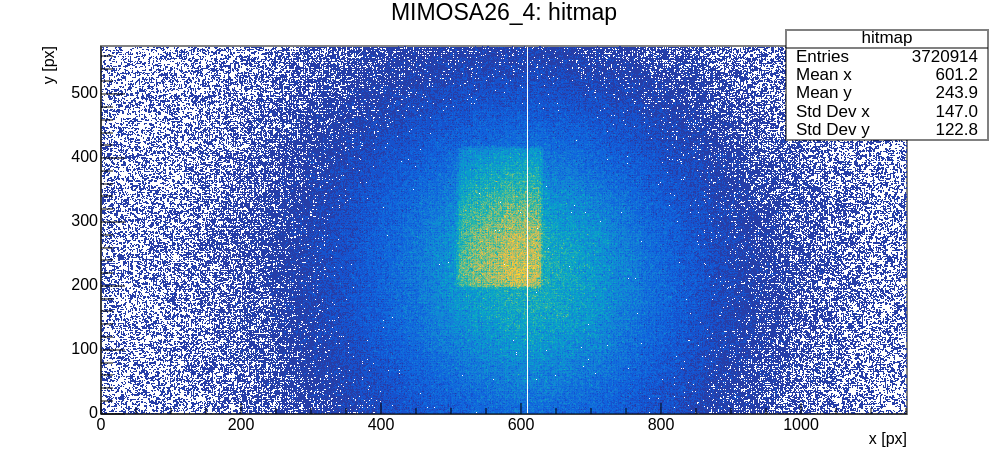
\includegraphics[width=.9\linewidth]{Images/appendix/hits_MIMOSA4.png}
    \caption{The hits heatmap of the MIMOSA plane n°4, which shows clearly the dead column of pixels, the source of the "empty line" that appeared in the data.}
    \label{fig:MIMOSA4_hits}
\end{figure}


\section{Mislabeled sensor}

One specific sensor had three channels connected to the readout board (IMEv3-W12-2x2-1.5E15, i.e. an array of 2x2 pads from IME, with fluence of \qty{1.5e15}{\neutroneq}), but, when plotting the outline of each pad, one of them did not match the expected configuration. Additionally, in the logbook of the test beam of May 2023, there was some contradicting information regarding the connected channels on the readout board. We suspect that the inconsistent sensor could actually be one of the pads of IMEv3-W12-\textbf{1x3}-1.5E15 but, for an unfortune coincidence, that sensor had no useful batches. %% (most likely cut out of the FEi4 ROI).
Therefore, it was not possible to confirm that two channels were simply swapped, and Channel4 of the IMEv3-W12-2x2-1.5E15 was excluded from the analysis.


\begin{figure}[h!tbp]
    \centering
    \includegraphics[width=.9\linewidth]{Images/appendix/2D_Sensors_605 S1 (pulseHeight cut)_overlapping_v3.png}
    \caption{This plot combines the 2D plot of the reconstructed tracks (after a \textit{pulse height cut}) of the three channels of IMEv3-W12-2x2-1.5E15. It is very obvious that Channel4 does not match the expected shape of a 2x2 grid, and it is very likely wrongly labeled.}
    \label{fig:mislabeled_sensor}
\end{figure}

%%% TODO: more description instead of just additional plots?
\section{Additonal plots}\label{sec:additional_plots}

\begin{figure}[h!tbp]
    \centering
    \subfloat[Using pulse height cut]{
        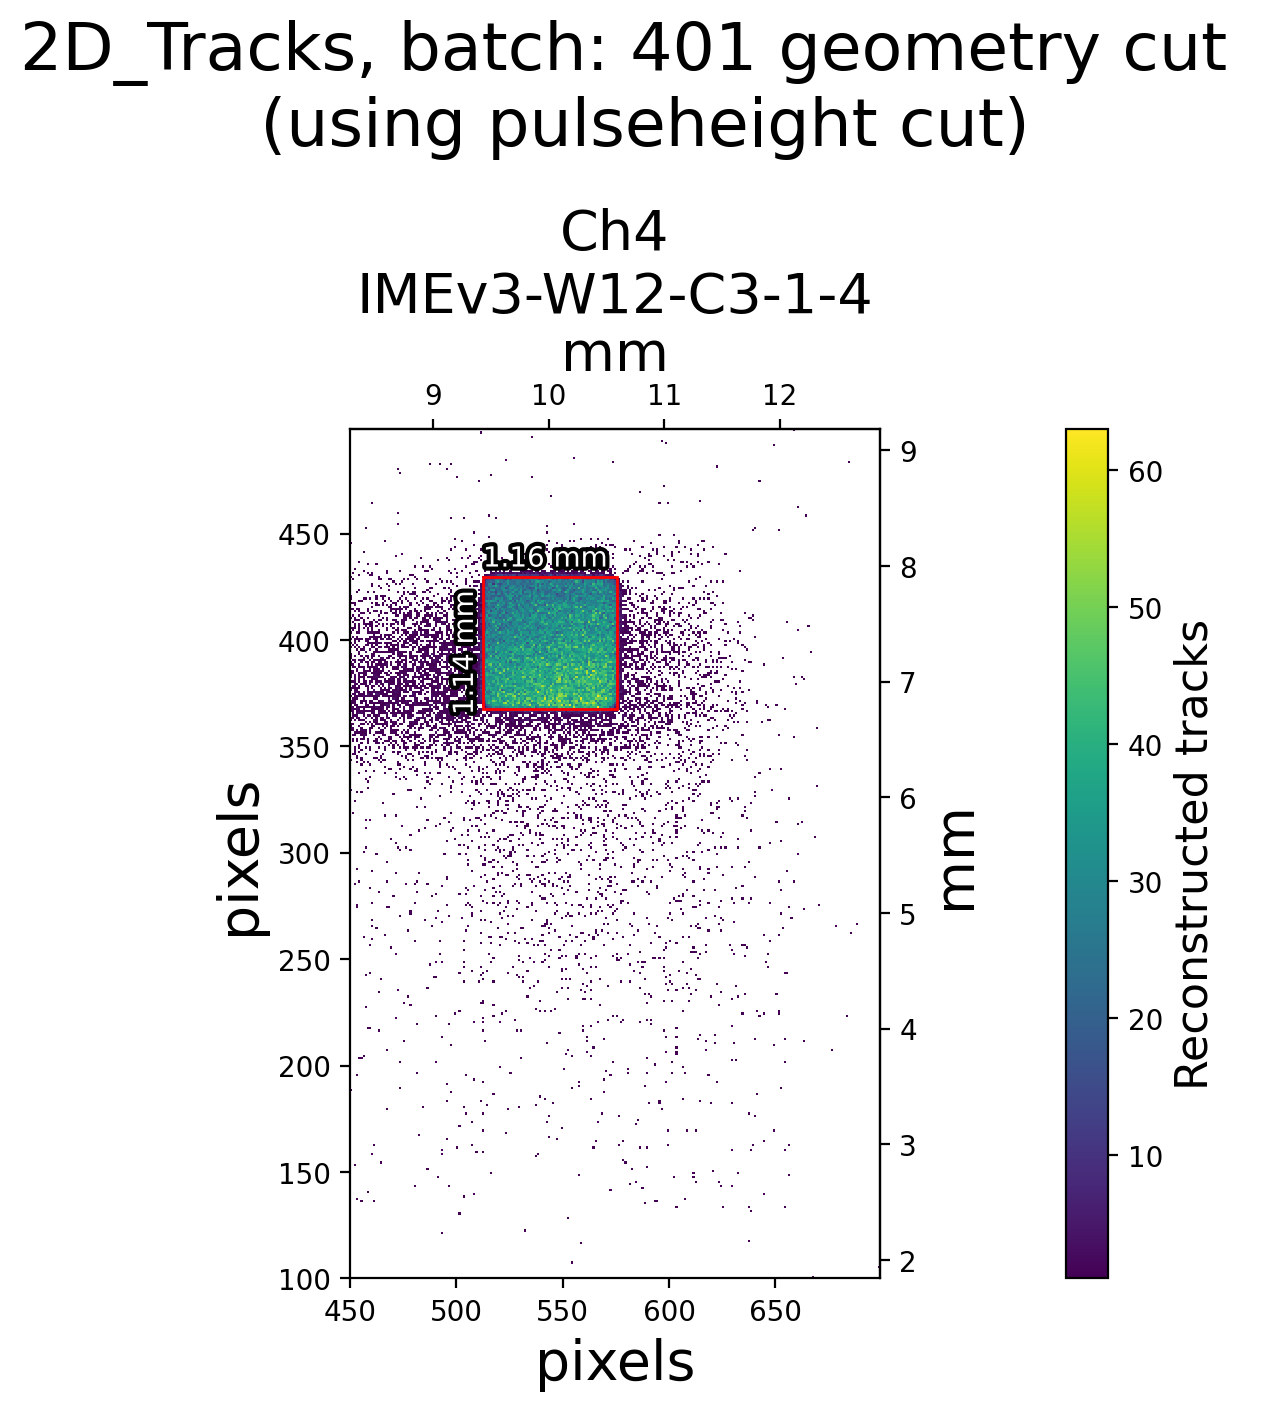
\includegraphics[width=.48\textwidth]{Images/appendix/2D_Tracks_401_S1 highlight geometry cut (using pulseHeight).png}
        \label{fig:geometry_cut_using_pulseHeight}}
    \hfill
    \centering
    \subfloat[Using time cut. Used only in the case of some irradiated sensors, when the noise was too high.]{
        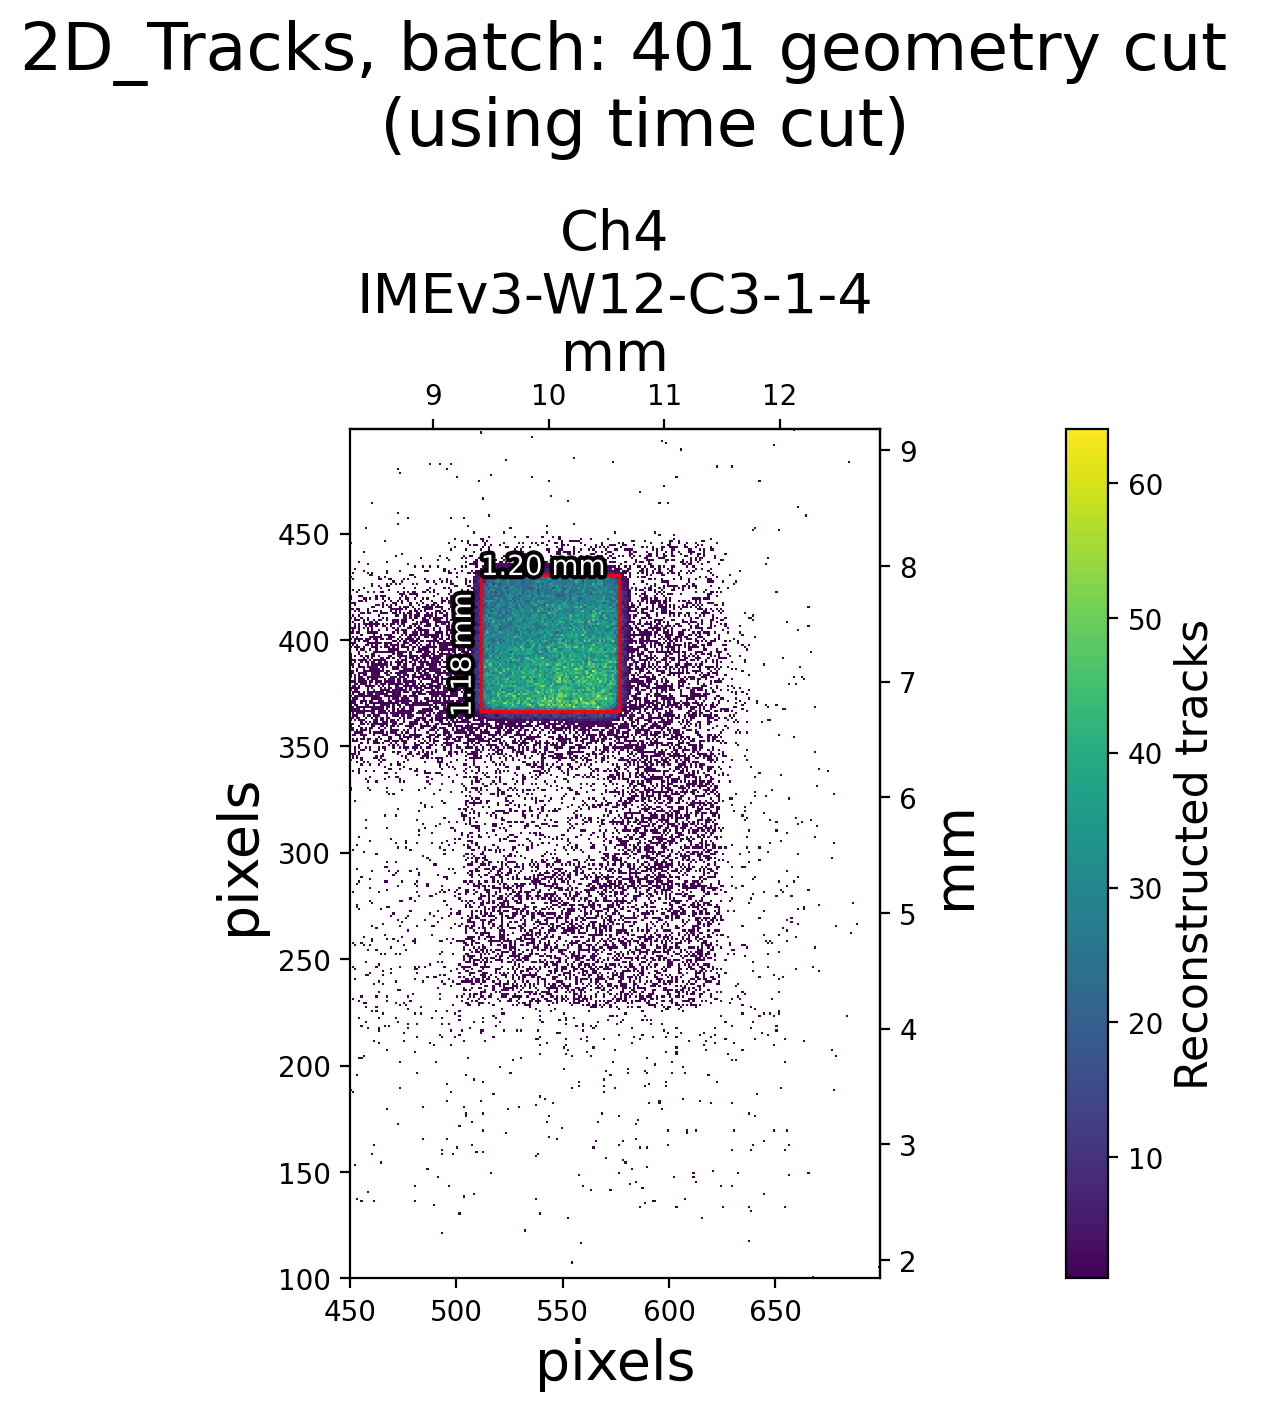
\includegraphics[width=.48\textwidth]{Images/appendix/2D_Tracks_401_S1 highlight geometry cut (using time).png}
        \label{fig:geometry_cut_using_time}}
    \caption{Example of the \textit{geometry cut} (red rectangles) obtained by applying a \textit{pulse height cut} (left) and a \textit{time cut} (left) to show that they produce comparable results. In practice, since all results were calculated inside the smaller \ \(0.5\times0.5\unit{\milli\meter^2}\) area, there were no real differences.}
    \label{fig:geometry_cut_comparison}
\end{figure}

\begin{figure}[h!tbp]
    \centering
    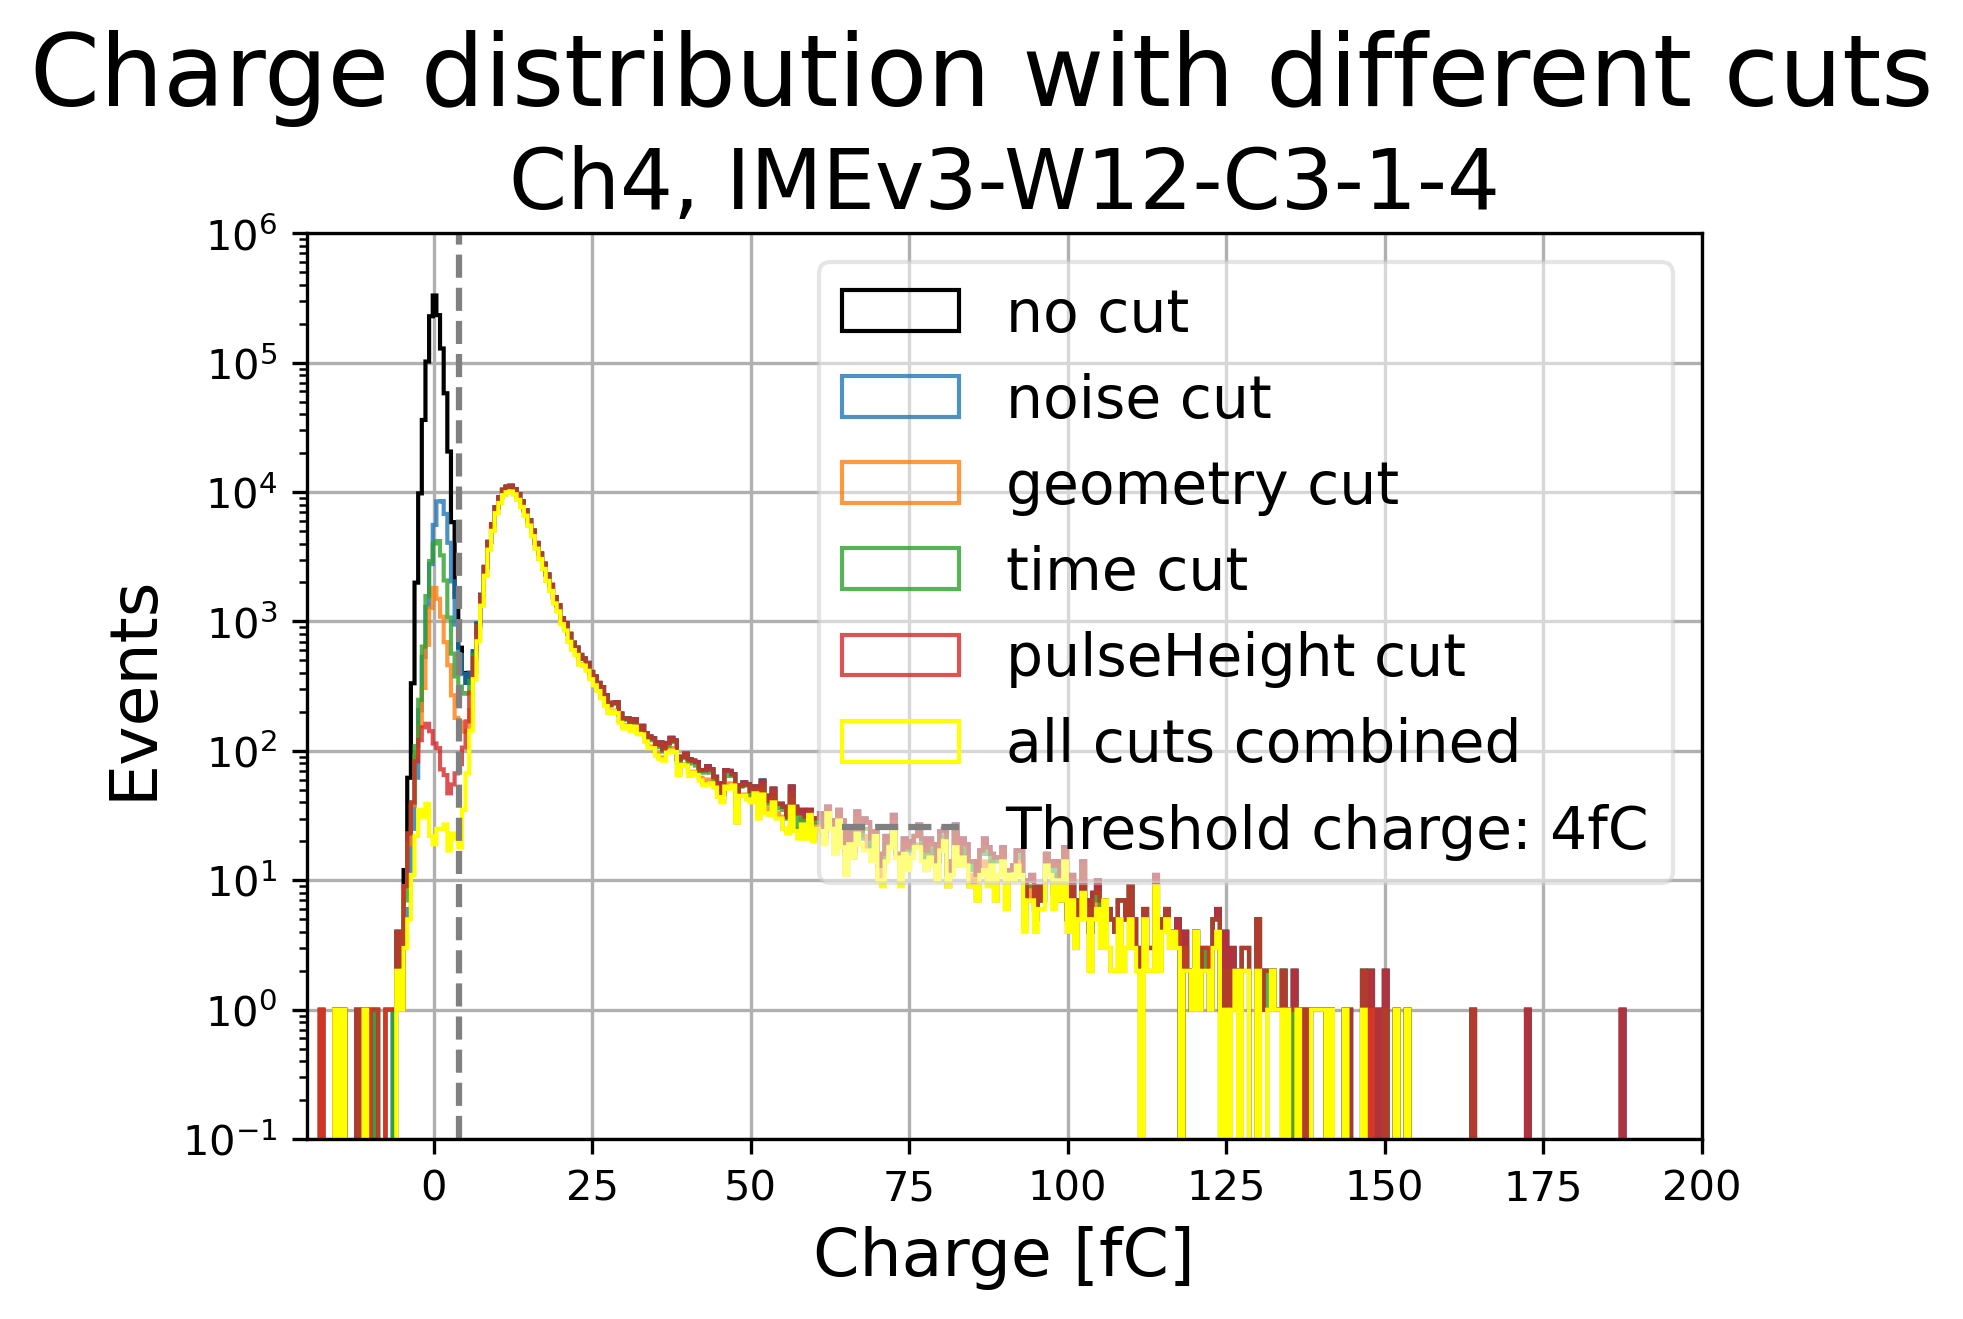
\includegraphics[width=0.7\linewidth]{Images/appendix/Charge_distribution_different_cuts_batch_401_S1_DUTs_3.png}
    \caption{The different quality cuts applied and their individual effect on the charge distribution}
    \label{fig:charge_plot_all_cuts}
\end{figure}

% \section{Sens}

% \begin{landscape}

% \begin{table}[h]
%     \caption{Complete list of the tested devices with additional details}
%     \label{tab:full_devices_tested}
%     \scriptsize
%         \begin{tabularx}{\textheight}{|l|l|l|l|l|l|l|l|X|}
%             \hline
%             \textbf{Device name} & \textbf{Vendor} & \textbf{Sensor ID} &  \begin{tabular}{@{}l@{}}\textbf{Pads,} \\ \textbf{used channels}\end{tabular} & \begin{tabular}{@{}l@{}}\textbf{Fluence} \\ \([n_{eq}/\si{cm^2}]\) \end{tabular} &\begin{tabular}{@{}l@{}} \textbf{Radiation} \\ \textbf{type} \end{tabular} & \textbf{Board name} & \begin{tabular}{@{}l@{}}\textbf{Board} \\ \textbf{channels} \end{tabular} & \textbf{Notes} \\
%             \hline
%             CNM-W4 & CNM & CNM-R15973-W4-D168 & single & 0 & - & JSI-B12 & - & reference \\ 
%             CNM-W5 & CNM & CNM-R15973-W5-D138 & single & 0 & - & JSI-B14 & - & reference \\ 
%             CNM-W5-1.5E15 & CNM & CNM-R15973-W5-D29 & single & \(\num{1.50E+15}\) & neutron & JSI-B5 & - & \\ 
%             CNM-W3-2.5E15 & CNM & CNM-R15973-W3-D29 & single & \(\num{2.50E+15}\) & neutron & JSI-PP1 & - & \\
%             USTC2.1-W17 & USTC & USTC2.1-W17-P6-A-2x2 & 2x2, 2 channels & 0 & - & CERN-3 & Ch1,Ch2 & \\
%             USTC2.1-W19 & USTC & USTC2.1-W19-P5-A-1x1 & single & 0 & - & CERN-3 & - & not tested \\
%             USTC2.1-W17-2E14 & USTC & USTC2.1-W17-P6-A-2x2 & 2x2, 1 channel & 0 & - & JSI-B2 & - & missing \\ 
%             IMEv3-W12-2x2 & IHEP & IMEv3-W12-C2-2-2 & 2x2, 2 channels & 0 & - & CERN-1 & Ch1,Ch2 &  \\ 
%             IMEv3-W12-1x3 & IHEP & IMEv3-W12-C3-1-4(and 5) & 1x3, 2 channels & 0 & - & CERN-1 & Ch3,Ch4 &  \\ 
%             IMEv3-W12-2x2-1.5E15 & IHEP & IMEv3-W12-B2-2-9-1 & 2x2, 3 channels & \(\num{1.50E+15}\) & neutron & CERN-2 & Ch0,Ch1,Ch2 &  \\ 
%             IMEv3-W16-1x3-1.5E15 & IHEP & IMEv3-W16-Q4-D4-1-4 & 1x3, 1 channel & \(\num{1.50E+15}\) & neutron & CERN-2 & Ch3 &  \\ 
%             IMEv2-W7-1E14 & IHEP & W7-II-C2-1-7IMEv2-W7Q2 & single & \(\num{1.00E+14}\) & proton & JSI-B6 & - &  \\ 
%             IMEv2-W7-6.5E14 & IHEP & W7-II-C2-1-7IMEv2-W7Q2 & single & \(\num{6.50E+14}\) & proton & JSI-PP4 & - &  \\ 
%             IMEv3-W16-8E14 & IHEP & IHEP-IMEv3-W16-Q4-D3-1-4 & single & \(\num{8.00E+14}\) & proton & JSI-B7 & - &  \\ 
%             IMEv3-W16-2.5E15 & IHEP & IHEP-IMEv3-W16-Q4-E3-1-4 & single & \(\num{2.50E+15}\) & neutron & JSI-B13 & - &  \\ 
%             \hline
%         \end{tabularx}
% \end{table}
% \end{landscape}

\FloatBarrier

\section{Table of results}

Here are reported the tables containing all the results, divided by sensor. The column "Batch" indicates the batch number, the oscilloscope ('S1' or 'S2') and the channel number; multiple entries of a single batch number refer to multiple connected pads. The batch numbered \(5031\) was originally numbered \(503\), but it was divided in two batches because there was a significant shift in the position of the DUTs. \(5032\) was later removed due to the redundancy and higher noise.

%% All the tables with the results:
%%% CNM-W4
\begin{table}[htbp]
    \scriptsize
    \centering
    \caption{Summary of the results for the sensor: CNM-W4.}
    \label{tab:results_CNM-W4}
    \begin{tabular}{cccccccccccc}
\toprule
 &  &  & MCP [V] & Temp. [°C] & Angle [°] & Volt. [V] & Charge [fC] & \(\pm\sigma\) [fC] & Time res. [ps] & \(\pm\sigma\) [ps] & Eff. \\
Batch &  &  &  &  &  &  &  &  &  &  &  \\
\midrule
199 & S2 & Ch3 & 2600 & -31.2 & 0 & -80 & 10.39 & 0.03 & 51.73 & 1.84 & 0.990 \\
301 & S2 & Ch3 & 2500 & 21.8 & 0 & -150 & 13.32 & 0.01 & 38.01 & 0.96 & 0.995 \\
401 & S2 & Ch3 & 2500 & -30.6 & 0 & -80 & 10.33 & 0.01 & 43.17 & 0.82 & 0.993 \\
402 & S2 & Ch3 & 2500 & -29.9 & 0 & -100 & 14.27 & 0.01 & 30.68 & 1.09 & 0.994 \\
407 & S2 & Ch3 & 2500 & -30.0 & 0 & -120 & 24.98 & 0.02 & 26.78 & 1.21 & 0.996 \\
408 & S2 & Ch3 & 2500 & 21.4 & 0 & -160 & 16.20 & 0.02 & 36.41 & 1.18 & 0.994 \\
409 & S2 & Ch3 & 2500 & 21.7 & 0 & -175 & 23.61 & 0.03 & 27.76 & 1.37 & 0.995 \\
410 & S2 & Ch3 & 2600 & 21.8 & 0 & -175 & 23.66 & 0.04 & 30.55 & 0.70 & 0.995 \\
411 & S2 & Ch3 & 2500 & -29.6 & 13 & -120 & 28.94 & 0.03 & 25.71 & 1.44 & 0.997 \\
413 & S2 & Ch3 & 2800 & -30.2 & 6 & -120 & 25.60 & 0.03 & 30.04 & 0.27 & 0.997 \\
414 & S2 & Ch3 & 2800 & -31.9 & 6 & -100 & 15.03 & 0.01 & 41.60 & 0.31 & 0.997 \\
\bottomrule
\end{tabular}

\end{table}

%%% CNM-W5
\begin{table}[htbp]
    \scriptsize
    \centering
    \caption{Summary of the results for the sensor: CNM-W5.}
    \label{tab:results_CNM-W5}
    \begin{tabular}{ccccccccccc}
\toprule
 &  &  & Temp. [°C] & Angle [°] & Volt. [V] & Charge [fC] & \(\pm\sigma\) [fC] & Time res. [ps] & \(\pm\sigma\) [ps] & Eff. \\
\midrule
409 & S2 & Ch2 & 21.7 & 0 & -195 & 17.31 & 0.02 & 27.11 & 1.39 & 0.994 \\
410 & S2 & Ch2 & 21.8 & 0 & -195 & 27.64 & 0.04 & 29.74 & 0.66 & 0.998 \\
408 & S2 & Ch2 & 21.4 & 0 & -185 & 13.63 & 0.02 & 33.27 & 1.24 & 0.995 \\
301 & S2 & Ch2 & 21.8 & 0 & -180 & 19.11 & 0.01 & 29.02 & 1.17 & 0.995 \\
407 & S2 & Ch2 & -30.0 & 0 & -135 & 22.99 & 0.01 & 27.78 & 1.16 & 0.997 \\
413 & S2 & Ch2 & -30.2 & 6 & -130 & 15.50 & 0.02 & 30.24 & 0.28 & 0.996 \\
411 & S2 & Ch2 & -29.6 & 13 & -130 & 28.67 & 0.03 & 26.11 & 1.39 & 0.996 \\
403 & S2 & Ch2 & -31.2 & 0 & -120 & 18.39 & 0.02 & 25.21 & 1.36 & 0.995 \\
414 & S2 & Ch2 & -31.9 & 6 & -120 & 11.85 & 0.01 & 34.14 & 0.28 & 0.997 \\
402 & S2 & Ch2 & -29.9 & 0 & -100 & 12.60 & 0.01 & 33.53 & 1.02 & 0.995 \\
401 & S2 & Ch2 & -30.6 & 0 & -80 & 9.75 & 0.01 & 44.43 & 0.80 & 0.994 \\
199 & S2 & Ch2 & -31.2 & 0 & -80 & 9.70 & 0.06 & 50.32 & 3.95 & 0.996 \\
\bottomrule
\end{tabular}

\end{table}

%%% CNM-W5-1.5E15
\begin{table}[htbp]
    \scriptsize
    \centering
    \caption{Summary of the results for the sensor: CNM-W5-1.5E15.}
    \label{tab:results_CNM-W5-1.5E15}
    \begin{tabular}{cccccccccccc}
\toprule
 &  &  & MCP [V] & Temp. [°C] & Angle [°] & Volt. [V] & Charge [fC] & \(\pm\sigma\) [fC] & Time res. [ps] & \(\pm\sigma\) [ps] & Eff. \\
Batch &  &  &  &  &  &  &  &  &  &  &  \\
\midrule
501 & S2 & Ch3 & 2800 & -26.7 & 0 & -400 & 2.37 & 0.01 & 56.80 & 0.60 & 0.306 \\
502 & S2 & Ch3 & 2800 & -26.6 & 0 & -450 & 3.07 & 0.01 & 53.18 & 0.44 & 0.476 \\
504 & S2 & Ch3 & 2800 & -33.2 & 0 & -550 & 6.46 & 0.01 & 37.42 & 0.28 & 0.948 \\
505 & S2 & Ch3 & 2800 & -33.1 & 0 & -600 & 10.54 & 0.01 & 31.17 & 0.27 & 0.988 \\
1201 & S1 & Ch3 & 2800 & 0.0 & 0 & -620 & 9.11 & 0.01 & 30.61 & 0.55 & 0.947 \\
1202 & S1 & Ch3 & 2800 & 0.0 & 0 & -640 & 11.14 & 0.03 & 28.84 & 0.52 & 0.963 \\
5031 & S2 & Ch3 & 2800 & -29.8 & 0 & -500 & 4.26 & 0.01 & 45.74 & 0.44 & 0.727 \\
\bottomrule
\end{tabular}

\end{table}

%%% CNM-W3-2.5E15
\begin{table}[htbp]
    \scriptsize
    \centering
    \caption{Summary of the results for the sensor: CNM-W3-2.5E15.}
    \label{tab:results_CNM-W3-2.5E15}
    \begin{tabular}{ccccccccccc}
\toprule
 &  &  & Temp. [°C] & Angle [°] & Volt. [V] & Charge [fC] & \(\pm\sigma\) [fC] & Time res. [ps] & \(\pm\sigma\) [ps] & Eff. \\
\midrule
1202 & S1 & Ch2 & 0.0 & 0 & -640 & 2.51 & 0.04 & 44.78 & 5.93 & 0.953 \\
1201 & S1 & Ch2 & 0.0 & 0 & -620 & 2.12 & 0.01 & 56.12 & 1.84 & 0.933 \\
605 & S2 & Ch3 & -31.0 & 0 & -600 & 2.65 & 0.00 & 62.29 & 1.62 & 0.943 \\
604 & S2 & Ch3 & -31.1 & 0 & -550 & 1.43 & 0.01 & 63.40 & 2.04 & 0.850 \\
603 & S2 & Ch3 & -31.0 & 0 & -500 & 1.90 & 0.00 & 56.00 & 2.09 & 0.817 \\
602 & S2 & Ch3 & -30.8 & 0 & -450 & 1.53 & 0.00 & 39.66 & 1.91 & 0.801 \\
601 & S2 & Ch3 & -31.0 & 0 & -400 & 1.57 & 0.01 & 31.02 & 1.98 & 0.777 \\
\bottomrule
\end{tabular}

\end{table}

%%% USTC2.1-W17
\begin{table}[htbp]
    \scriptsize
    \centering
    \caption{Summary of the results for the sensor: USTC2.1-W17.}
    \label{tab:results_USTC2.1-W17}
    \begin{tabular}{cccccccccccc}
\toprule
 &  &  & MCP [V] & Temp. [°C] & Angle [°] & Volt. [V] & Charge [fC] & \(\pm\sigma\) [fC] & Time res. [ps] & \(\pm\sigma\) [ps] & Eff. \\
Batch &  &  &  &  &  &  &  &  &  &  &  \\
\midrule
301 & S1 & Ch2 & 2500 & 21.8 & 0 & -120 & 11.00 & 0.01 & 61.70 & 0.79 & 0.994 \\
 &  & Ch3 & 2500 & 21.8 & 0 & -120 & 11.51 & 0.01 & 55.00 & 0.85 & 0.996 \\
401 & S1 & Ch2 & 2500 & -30.6 & 0 & -80 & 17.02 & 0.01 & 52.38 & 0.74 & 0.995 \\
 &  & Ch3 & 2500 & -30.6 & 0 & -80 & 17.72 & 0.01 & 46.48 & 0.80 & 0.996 \\
402 & S1 & Ch2 & 2500 & -29.9 & 0 & -90 & 19.44 & 0.01 & 47.40 & 0.81 & 0.996 \\
 &  & Ch3 & 2500 & -29.9 & 0 & -90 & 20.19 & 0.01 & 43.01 & 0.88 & 0.996 \\
403 & S1 & Ch2 & 2500 & -31.2 & 0 & -100 & 23.89 & 0.02 & 41.34 & 0.96 & 0.996 \\
 &  & Ch3 & 2500 & -31.2 & 0 & -100 & 24.91 & 0.02 & 39.14 & 1.00 & 0.996 \\
407 & S1 & Ch2 & 2500 & -30.0 & 0 & -105 & 25.28 & 0.01 & 44.70 & 0.81 & 0.997 \\
 &  & Ch3 & 2500 & -30.0 & 0 & -105 & 26.78 & 0.02 & 40.76 & 0.88 & 0.997 \\
408 & S1 & Ch2 & 2500 & 21.4 & 0 & -150 & 16.17 & 0.02 & 53.10 & 1.06 & 0.996 \\
 &  & Ch3 & 2500 & 21.4 & 0 & -150 & 16.92 & 0.02 & 49.03 & 1.18 & 0.996 \\
409 & S1 & Ch2 & 2500 & 21.7 & 0 & -165 & 20.64 & 0.02 & 46.65 & 1.08 & 0.996 \\
 &  & Ch3 & 2500 & 21.7 & 0 & -165 & 21.89 & 0.02 & 44.83 & 1.14 & 0.997 \\
410 & S1 & Ch2 & 2600 & 21.8 & 0 & -165 & 20.65 & 0.03 & 41.31 & 0.77 & 0.995 \\
 &  & Ch3 & 2600 & 21.8 & 0 & -165 & 21.90 & 0.03 & 40.87 & 0.86 & 0.996 \\
413 & S1 & Ch2 & 2800 & -30.2 & 6 & -105 & 26.48 & 0.03 & 37.80 & 0.34 & 0.997 \\
 &  & Ch3 & 2800 & -30.2 & 6 & -105 & 28.10 & 0.03 & 36.34 & 0.33 & 0.997 \\
414 & S1 & Ch2 & 2800 & -31.9 & 6 & -100 & 25.20 & 0.02 & 38.97 & 0.35 & 0.997 \\
 &  & Ch3 & 2800 & -31.9 & 6 & -100 & 26.61 & 0.02 & 37.15 & 0.34 & 0.997 \\
\bottomrule
\end{tabular}

\end{table}

%%% IMEv3-W12-2x2
\begin{table}[htbp]
    \scriptsize
    \centering
    \caption{Summary of the results for the sensor: IMEv3-W12-2x2.}
    \label{tab:results_IMEv3-W12-2x2}
    \begin{tabular}{ccccccccccc}
\toprule
 &  &  & Temp. [°C] & Angle [°] & Volt. [V] & Charge [fC] & \(\pm\sigma\) [fC] & Time res. [ps] & \(\pm\sigma\) [ps] & Eff. \\
\midrule
199 & S1 & Ch2 & -31.2 & 0 & -80 & 13.75 & 0.09 & 77.22 & 5.17 & 0.997 \\
 &  & Ch3 & -31.2 & 0 & -80 & 14.00 & 0.09 & 69.80 & 2.70 & 0.993 \\
201 & S1 & Ch2 & -31.8 & 0 & -80 & 13.97 & 0.01 & 50.30 & 0.91 & 0.997 \\
 &  & Ch3 & -31.8 & 0 & -80 & 14.23 & 0.02 & 51.82 & 0.94 & 0.997 \\
202 & S1 & Ch2 & -32.5 & 0 & -90 & 16.38 & 0.01 & 46.06 & 0.91 & 0.997 \\
 &  & Ch3 & -32.5 & 0 & -90 & 16.48 & 0.02 & 49.11 & 0.92 & 0.997 \\
203 & S1 & Ch2 & -32.6 & 0 & -100 & 19.64 & 0.02 & 42.70 & 1.06 & 0.996 \\
 &  & Ch3 & -32.6 & 0 & -100 & 19.45 & 0.03 & 45.80 & 1.09 & 0.995 \\
204 & S1 & Ch2 & -30.3 & 0 & -125 & 49.00 & 0.08 & 42.00 & 0.96 & 1.000 \\
205 & S1 & Ch2 & -28.2 & 13 & -125 & 46.13 & 0.05 & 21.43 & 1.55 & 0.999 \\
206 & S1 & Ch2 & -27.9 & 13 & -100 & 19.94 & 0.02 & 36.70 & 1.18 & 0.998 \\
 &  & Ch3 & -27.9 & 13 & -100 & 20.30 & 0.03 & 35.99 & 1.20 & 0.997 \\
\bottomrule
\end{tabular}

\end{table}


%%% IMEv3-W12-1x3
\begin{table}[htbp]
    \scriptsize
    \centering
    \caption{Summary of the results for the sensor: IMEv3-W12-1x3}
    \label{tab:results_IMEv3-W12-1x3}
    \begin{tabular}{cccccccccccc}
\toprule
 &  &  & MCP [V] & Temp. [°C] & Angle [°] & Volt. [V] & Charge [fC] & \(\pm\sigma\) [fC] & Time res. [ps] & \(\pm\sigma\) [ps] & Eff. \\
Batch &  &  &  &  &  &  &  &  &  &  &  \\
\midrule
199 & S1 & Ch4 & 2600 & -31.2 & 0 & -80 & 11.53 & 0.04 & 56.62 & 1.98 & 0.995 \\
 & S2 & Ch4 & 2600 & -31.2 & 0 & -80 & 13.65 & 0.04 & 49.81 & 1.82 & 0.987 \\
301 & S2 & Ch4 & 2500 & 21.8 & 0 & -100 & 7.65 & 0.01 & 59.25 & 0.87 & 0.986 \\
401 & S1 & Ch4 & 2500 & -30.6 & 0 & -80 & 11.39 & 0.01 & 47.72 & 0.88 & 0.994 \\
 & S2 & Ch4 & 2500 & -30.6 & 0 & -80 & 13.60 & 0.01 & 41.02 & 0.87 & 0.995 \\
402 & S1 & Ch4 & 2500 & -29.9 & 0 & -90 & 12.93 & 0.01 & 43.20 & 0.98 & 0.994 \\
 & S2 & Ch4 & 2500 & -29.9 & 0 & -90 & 15.44 & 0.01 & 36.92 & 0.97 & 0.995 \\
403 & S1 & Ch4 & 2500 & -31.2 & 0 & -100 & 15.47 & 0.02 & 39.13 & 1.14 & 0.994 \\
 & S2 & Ch4 & 2500 & -31.2 & 0 & -100 & 18.55 & 0.02 & 31.76 & 1.17 & 0.995 \\
407 & S1 & Ch4 & 2500 & -30.0 & 0 & -125 & 29.73 & 0.03 & 32.29 & 1.09 & 0.997 \\
 & S2 & Ch4 & 2500 & -30.0 & 0 & -125 & 35.66 & 0.03 & 21.31 & 1.50 & 0.997 \\
408 & S1 & Ch4 & 2500 & 21.4 & 0 & -160 & 13.64 & 0.03 & 42.42 & 1.34 & 0.995 \\
 & S2 & Ch4 & 2500 & 21.4 & 0 & -160 & 16.50 & 0.02 & 32.42 & 1.33 & 0.995 \\
409 & S1 & Ch4 & 2500 & 21.7 & 0 & -160 & 13.58 & 0.03 & 40.82 & 1.35 & 0.990 \\
 & S2 & Ch4 & 2500 & 21.7 & 0 & -160 & 16.39 & 0.02 & 32.17 & 1.32 & 0.995 \\
410 & S1 & Ch4 & 2600 & 21.8 & 0 & -160 & 13.56 & 0.04 & 39.80 & 1.04 & 0.990 \\
 & S2 & Ch4 & 2600 & 21.8 & 0 & -160 & 16.46 & 0.03 & 34.05 & 0.82 & 0.994 \\
411 & S1 & Ch4 & 2500 & -29.6 & 13 & -125 & 34.25 & 0.07 & 33.41 & 1.33 & 0.997 \\
 & S2 & Ch4 & 2500 & -29.6 & 13 & -125 & 41.26 & 0.07 & 22.30 & 1.63 & 0.997 \\
413 & S1 & Ch4 & 2800 & -30.2 & 6 & -125 & 29.16 & 0.04 & 26.17 & 0.30 & 0.998 \\
 & S2 & Ch4 & 2800 & -30.2 & 6 & -125 & 36.46 & 0.05 & 25.58 & 0.27 & 0.997 \\
414 & S1 & Ch4 & 2800 & -31.9 & 6 & -100 & 15.75 & 0.01 & 34.28 & 0.34 & 0.996 \\
 & S2 & Ch4 & 2800 & -31.9 & 6 & -100 & 18.96 & 0.02 & 33.66 & 0.27 & 0.995 \\
\bottomrule
\end{tabular}

\end{table}

%%% IMEv3-W12-2x2-1.5E15
\begin{table}[htbp]
    \scriptsize
    \centering
    \caption{Summary of the results for the sensor: IMEv3-W12-2x2-1.5E15}
    \label{tab:results_IMEv3-W12-2x2-1.5E15}
    \begin{tabular}{cccccccccccc}
\toprule
 &  &  & MCP [V] & Temp. [°C] & Angle [°] & Volt. [V] & Charge [fC] & \(\pm\sigma\) [fC] & Time res. [ps] & \(\pm\sigma\) [ps] & Eff. \\
Batch &  &  &  &  &  &  &  &  &  &  &  \\
\midrule
601 & S1 & Ch2 & 2800 & -31.0 & 0 & -300 & 4.46 & 0.01 & 47.37 & 0.39 & 0.764 \\
 &  & Ch3 & 2800 & -31.0 & 0 & -300 & 4.69 & 0.01 & 48.30 & 0.43 & 0.792 \\
602 & S1 & Ch2 & 2800 & -30.8 & 0 & -350 & 5.96 & 0.02 & 39.56 & 0.49 & 0.932 \\
 &  & Ch3 & 2800 & -30.8 & 0 & -350 & 7.84 & 0.00 & 41.96 & 0.56 & 0.940 \\
603 & S1 & Ch2 & 2800 & -31.0 & 0 & -400 & 8.68 & 0.01 & 34.95 & 0.34 & 0.984 \\
 &  & Ch3 & 2800 & -31.0 & 0 & -400 & 9.10 & 0.01 & 36.03 & 0.38 & 0.984 \\
604 & S1 & Ch2 & 2800 & -31.1 & 0 & -450 & 12.24 & 0.01 & 30.84 & 0.30 & 0.987 \\
 &  & Ch3 & 2800 & -31.1 & 0 & -450 & 12.75 & 0.02 & 31.60 & 0.32 & 0.989 \\
605 & S1 & Ch2 & 2800 & -31.0 & 0 & -490 & 16.37 & 0.03 & 30.24 & 0.38 & 0.985 \\
 &  & Ch3 & 2800 & -31.0 & 0 & -490 & 17.09 & 0.03 & 30.71 & 0.43 & 0.985 \\
701 & S1 & Ch2 & 2800 & -31.3 & 14 & -490 & 19.57 & 0.02 & 29.02 & 0.24 & 0.988 \\
 &  & Ch3 & 2800 & -31.3 & 14 & -490 & 20.35 & 0.02 & 30.29 & 0.26 & 0.987 \\
702 & S1 & Ch2 & 2800 & -31.1 & 14 & -450 & 14.06 & 0.02 & 30.22 & 0.31 & 0.987 \\
 &  & Ch3 & 2800 & -31.1 & 14 & -450 & 14.70 & 0.02 & 31.96 & 0.34 & 0.988 \\
1001 & S1 & Ch2 & 2800 & -31.5 & 6 & -490 & 18.63 & 0.02 & 29.43 & 0.30 & 0.988 \\
 &  & Ch3 & 2800 & -31.5 & 6 & -490 & 19.29 & 0.03 & 30.22 & 0.32 & 0.989 \\
1002 & S1 & Ch2 & 2800 & -31.6 & 6 & -450 & 13.78 & 0.02 & 31.16 & 0.30 & 0.987 \\
 &  & Ch3 & 2800 & -31.6 & 6 & -450 & 14.40 & 0.02 & 31.21 & 0.33 & 0.988 \\
\bottomrule
\end{tabular}

\end{table}


%%% IMEv2-W7-1E14
\begin{table}[htbp]
    \scriptsize
    \centering
    \caption{Summary of the results for the sensor: IMEv2-W7-1E14}
    \label{tab:results_IMEv2-W7-1E14}
    \begin{tabular}{ccccccccccc}
\toprule
 &  &  & Temp. [°C] & Angle [°] & Volt. [V] & Charge [fC] & \(\pm\sigma\) [fC] & Time res. [ps] & \(\pm\sigma\) [ps] & Eff. \\
\midrule
501 & S2 & Ch2 & -26.7 & 0 & -80 & 5.11 & 0.01 & 73.01 & 0.39 & 0.990 \\
502 & S2 & Ch2 & -26.6 & 0 & -100 & 6.39 & 0.01 & 55.28 & 0.28 & 0.992 \\
504 & S2 & Ch2 & -33.2 & 0 & -150 & 13.91 & 0.01 & 30.18 & 0.24 & 0.993 \\
801 & S2 & Ch3 & -31.2 & 14 & -150 & 13.71 & 0.02 & 32.03 & 0.36 & 0.982 \\
802 & S2 & Ch3 & -31.2 & 14 & -120 & 8.58 & 0.01 & 43.36 & 0.43 & 0.983 \\
1001 & S2 & Ch3 & -31.5 & 6 & -150 & 11.43 & 0.02 & 30.83 & 0.34 & 0.981 \\
1002 & S2 & Ch3 & -31.6 & 6 & -120 & 9.14 & 0.02 & 42.64 & 0.53 & 0.984 \\
1102 & S2 & Ch3 & -31.1 & 6 & -150 & 14.33 & 0.02 & 31.91 & 0.30 & 0.987 \\
5031 & S2 & Ch2 & -29.8 & 0 & -120 & 8.07 & 0.01 & 44.77 & 0.34 & 0.990 \\
\bottomrule
\end{tabular}

\end{table}

%%% IMEv2-W7-6.5E14
\begin{table}[htbp]
    \scriptsize
    \centering
    \caption{Summary of the results for the sensor: {IMEv2-W7-6.5E14}}
    \label{tab:results_IMEv2-W7-6.5E14}
    \begin{tabular}{cccccccccccc}
\toprule
 &  &  & MCP [V] & Temp. [°C] & Angle [°] & Volt. [V] & Charge [fC] & \(\pm\sigma\) [fC] & Time res. [ps] & \(\pm\sigma\) [ps] & Eff. \\
Batch &  &  &  &  &  &  &  &  &  &  &  \\
\midrule
502 & S1 & Ch2 & 2800 & -26.6 & 0 & -250 & 2.65 & 0.01 & 73.86 & 0.76 & 0.250 \\
504 & S1 & Ch2 & 2800 & -33.2 & 0 & -350 & 4.91 & 0.02 & 52.48 & 0.37 & 0.747 \\
505 & S1 & Ch2 & 2800 & -33.1 & 0 & -400 & 7.31 & 0.02 & 40.40 & 0.27 & 0.943 \\
901 & S1 & Ch2 & 2800 & -31.3 & 13 & -400 & 9.68 & 0.02 & 36.67 & 0.32 & 0.977 \\
902 & S1 & Ch2 & 2800 & -31.3 & 13 & -350 & 5.81 & 0.02 & 45.56 & 0.49 & 0.876 \\
1101 & S1 & Ch2 & 2800 & -31.0 & 6 & -400 & 4.77 & 0.03 & 50.27 & 0.74 & 0.744 \\
1102 & S1 & Ch2 & 2800 & -31.1 & 6 & -350 & 4.54 & 0.00 & 58.41 & 1.15 & 0.554 \\
5031 & S1 & Ch2 & 2800 & -29.8 & 0 & -300 & 3.65 & 0.00 & 65.44 & 0.85 & 0.425 \\
\bottomrule
\end{tabular}

\end{table}

%%% IMEv3-W16-8E14
\begin{table}[htbp]
    \scriptsize
    \centering
    \caption{Summary of the results for the sensor: IMEv3-W16-8E14}
    \label{tab:results_IMEv3-W16-8E14}
    \begin{tabular}{ccccccccccc}
\toprule
 &  &  & Temp. [°C] & Angle [°] & Volt. [V] & Charge [fC] & \(\pm\sigma\) [fC] & Time res. [ps] & \(\pm\sigma\) [ps] & Eff. \\
\midrule
501 & S1 & Ch3 & -26.7 & 0 & -200 & 5.23 & 0.00 & 54.49 & 0.29 & 0.992 \\
502 & S1 & Ch3 & -26.6 & 0 & -250 & 7.39 & 0.01 & 41.67 & 0.22 & 0.994 \\
504 & S1 & Ch3 & -33.2 & 0 & -350 & 16.70 & 0.02 & 30.04 & 0.24 & 0.993 \\
505 & S1 & Ch3 & -33.1 & 0 & -370 & 17.86 & 0.03 & 33.27 & 0.25 & 0.976 \\
801 & S2 & Ch2 & -31.2 & 14 & -360 & 13.90 & 0.03 & 32.05 & 0.37 & 0.976 \\
802 & S2 & Ch2 & -31.2 & 14 & -340 & 12.73 & 0.02 & 30.07 & 0.34 & 0.977 \\
1001 & S2 & Ch2 & -31.5 & 6 & -360 & 18.24 & 0.03 & 32.29 & 0.26 & 0.978 \\
1002 & S2 & Ch2 & -31.6 & 6 & -340 & 16.69 & 0.02 & 29.88 & 0.29 & 0.981 \\
1101 & S2 & Ch2 & -31.0 & 6 & -360 & 18.23 & 0.02 & 32.02 & 0.24 & 0.977 \\
1102 & S2 & Ch2 & -31.1 & 6 & -340 & 16.71 & 0.02 & 30.22 & 0.27 & 0.979 \\
5031 & S1 & Ch3 & -29.8 & 0 & -300 & 11.82 & 0.01 & 32.75 & 0.29 & 0.992 \\
\bottomrule
\end{tabular}

\end{table}

% %%% IMEv3-W16-1x3-1.5E15  this one only has one good batch, it was excluded

%%% IMEv3-W16-2.5E15
\begin{table}[htbp]
    \scriptsize
    \centering
    \caption{IMEv3-W16-2.5E15}
    \label{tab:results_IMEv3-W16-2.5E15}
    \begin{tabular}{cccccccccccc}
\toprule
 &  &  & MCP [V] & Temp. [°C] & Angle [°] & Volt. [V] & Charge [fC] & \(\pm\sigma\) [fC] & Time res. [ps] & \(\pm\sigma\) [ps] & Eff. \\
Batch &  &  &  &  &  &  &  &  &  &  &  \\
\midrule
501 & S1 & Ch4 & 2800 & -26.7 & 0 & -400 & 2.21 & 0.01 & 57.90 & 0.68 & 0.211 \\
502 & S1 & Ch4 & 2800 & -26.6 & 0 & -450 & 2.50 & 0.00 & 58.32 & 0.57 & 0.305 \\
5031 & S1 & Ch4 & 2800 & -29.8 & 0 & -500 & 3.08 & 0.01 & 53.51 & 0.70 & 0.445 \\
\bottomrule
\end{tabular}

\end{table}

